\subsection{Membrane-magnet system}
The magnet needs to be suspended to allow it to move freely only on the z-axis, to achieve this we need a structure that constrains the lateral motion of the magnet and needs to also be able to vibrate freely with it.
To do this we can use a flexible membrane that can deform under the magnetic field generated by the coil and the magnet. 

As an example, we will analyze the membrane structure of the last type of prototype we implemented %\ref{sec:Flexible_Mat_Prototypes}
\begin{figure}
    \centering
    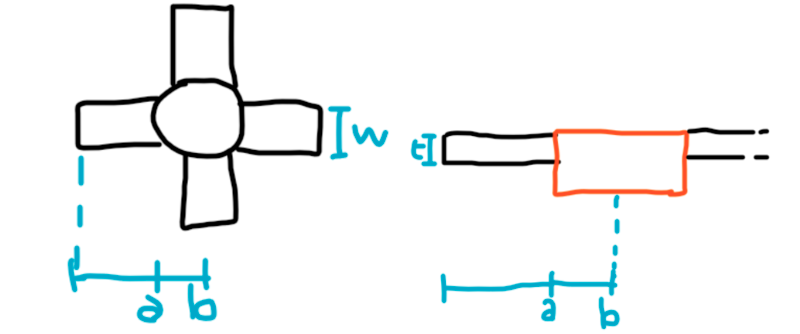
\includegraphics[scale=0.4]{Chapters/Chapter2/Modelling_of_Entire_System/Figures/membrane.png} % TODO: Change image with svg
    \caption[Membrane structure]{Membrane structure of the last prototype.}
    \label{fig:Membrane_structure}
\end{figure}

This membrane is a simple Celtic-cross structure made of thin silicone integrated with the entire structure of the device,
the membrane is built with a central cylindrical chamber used to trap the magnet in the center of the cross.
\begin{figure}
    \centering
    \resizebox{.9\linewidth}{!}{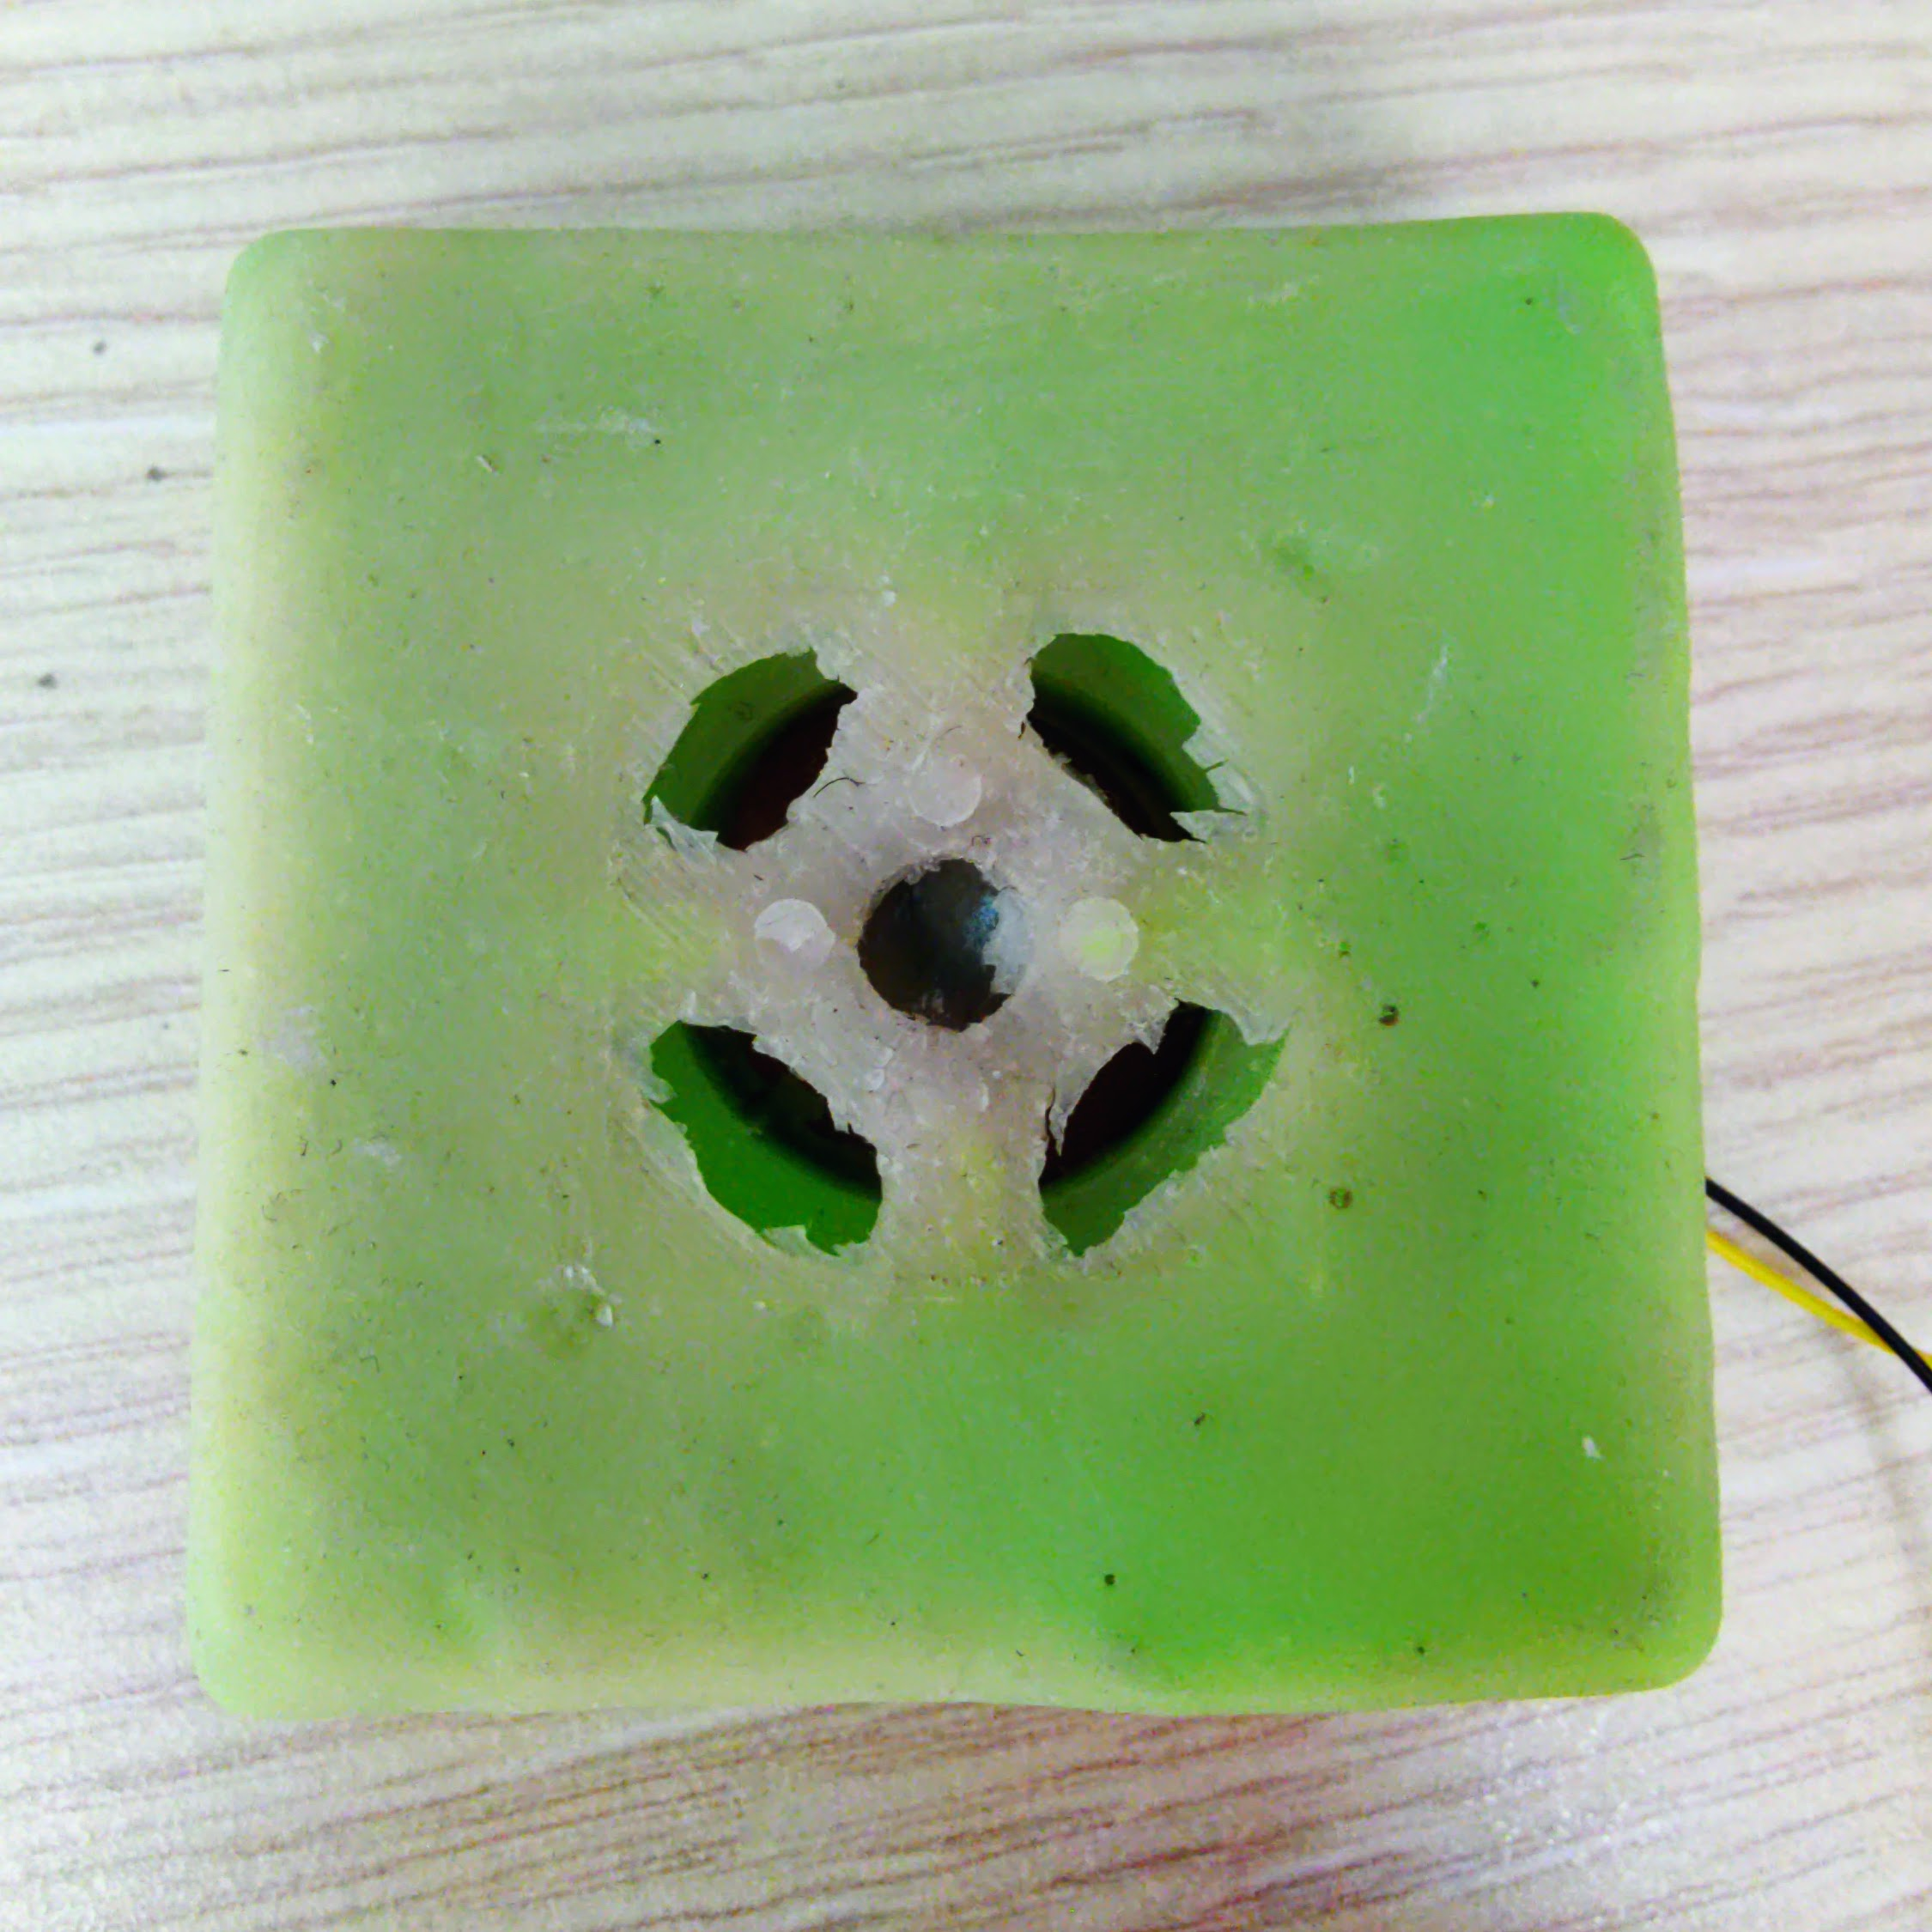
\includegraphics{Chapters/Chapter2/Modelling_of_Entire_System/Figures/Flexible_mat_small_top.jpg}}
    \caption[Membrane mat]{Membrane of the last prototype with the magnet trapped in the center.}
    \label{fig:Membrane_trap}
\end{figure}

The membrane can be modeled as a mass-spring-damper system.
\begin{figure}
    \centering
    \resizebox{.9\linewidth}{!}{
        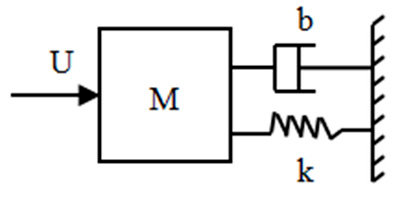
\includegraphics[scale = 0.6]{Chapters/Chapter2/Modelling_of_Entire_System/Figures/membrane_mech_model.png}
        \begin{tikzpicture}
    \begin{scope}[every node/.style={bgelement}]
    \node (start) at (0,0) {};
    \node[right=1 of start] (w) {1: Mech};
    \node[above=1 of w] (Cm) {C: $\frac{1}{ks_{membr}}$};
    \node[below=1 of w] (Rm) {R: b\textsubscript{membr}};
    \node[right=1 of w] (Im) {I: M\textsubscript{magnet}};
    \end{scope}
    \draw[bonds]
    (start) edge [e_in, flow={i}, effort={V}] (w)
    (w) edge [e_out] (Cm)
    (w) edge [e_in] (Rm)
    (w) edge [e_in] (Im);
\end{tikzpicture}    
    }
    \caption{Bond graph of the membrane-magnet system.}
    \label{fig:Membrane_bond_graph}
\end{figure}

\subsubsection{Membrane stiffness}
The membrane stiffness can be calculated using Young's modulus of the material and the geometry of the membrane.
Each arm of the cross can be considered as a cantilever beam, the stiffness of a cantilever beam can be calculated as:
\begin{equation}
    ks = \frac{3 E I_x}{L^3}
\end{equation}
Where:
\begin{itemize}
    \item $ks$ is the stiffness of the membrane's arm [N/m]
    \item $E$ is the Young's modulus of the material [Pa]
    \item $I$ is the second moment of inertia of the arm [m\textsuperscript{4}]
    \item $L$ is the length of the arm [m]
\end{itemize}

The arm can be simplified as a parallelepiped with a rectangular section, and the second moment of inertia on x can be calculated as:
\begin{equation}
    I_x = \frac{w t^3}{12}
\end{equation}
Where:
\begin{itemize}
    \item $I_x$ is the second moment of inertia on the x-axis [m\textsuperscript{4}]
    \item $w$ is the width of one membrane arm as in figure \ref{fig:Membrane_structure}[m]
    \item $t$ is the thickness of the membrane as in figure \ref{fig:Membrane_structure}[m]
\end{itemize}

\begin{figure}
    \centering
    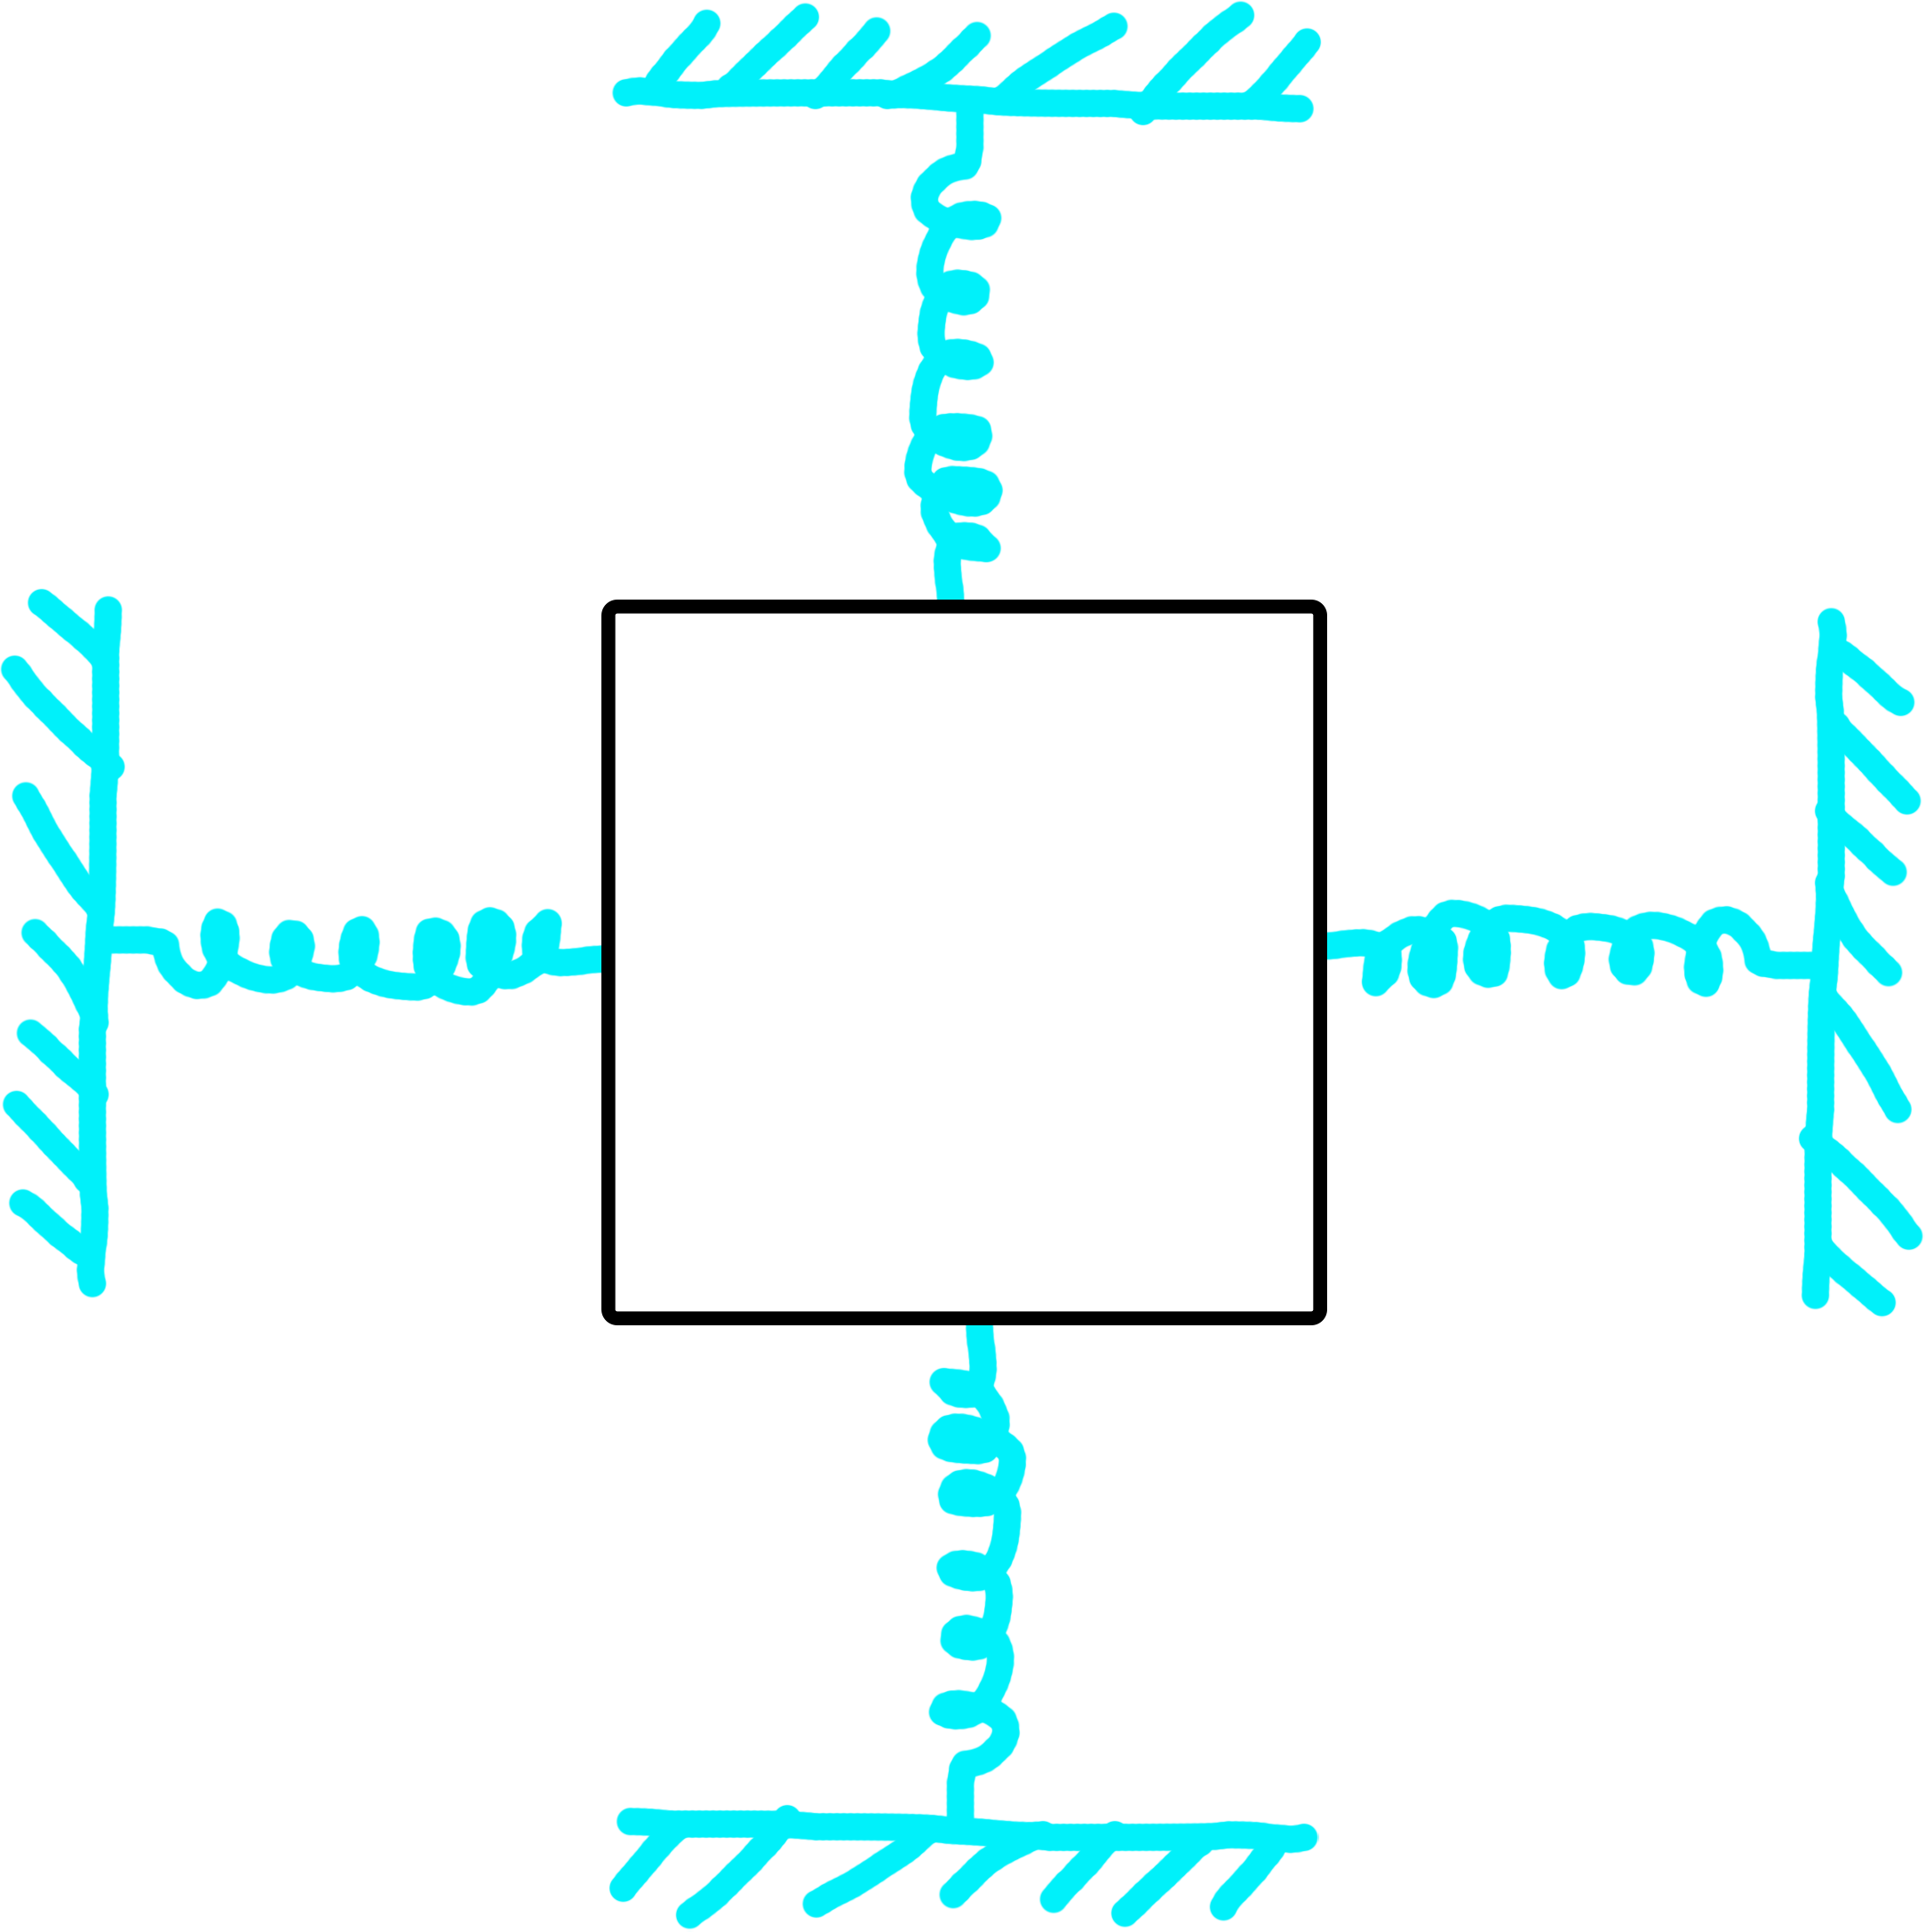
\includegraphics[scale=0.4]{Chapters/Chapter2/Modelling_of_Entire_System/Figures/4_arms_springs.png} % TODO: Change image with svg
    \caption{Membrane arms parallel springs.}
    \label{fig:Membrane_springs}
\end{figure}
Then we can consider the 4 arms as 4 springs in parallel, the total stiffness of the membrane can be calculated as:
\begin{equation}
    ks_{membr} = 4 ks
\end{equation}


\subsubsection{Membrane damping}
The damping for a cantilever beam is neglectable, so we can remove the resistive component from the mechanical model.
\begin{figure}
    \centering
    \resizebox{.9\linewidth}{!}{
        \begin{tikzpicture}
    \begin{scope}[every node/.style={bgelement}]
    \node (start) at (0,0) {};
    \node[right=1 of start] (w) {1: Mech};
    \node[above=1 of w] (Cm) {C: $\frac{1}{ks_{membr}}$};
    \node[right=1 of w] (Im) {I: M\textsubscript{magnet}};
    \end{scope}
    \draw[bonds]
    (start) edge [e_in, flow={i}, effort={V}] (w)
    (w) edge [e_out] (Cm)
    (w) edge [e_in] (Im);
\end{tikzpicture}    
    }
    \caption{Final mechanical bond-graph of the membrane and magnet.}
    \label{fig:Membrane_bond graph_without_damping}
\end{figure}

